\documentclass[10pt]{article}
\usepackage[margin=1.2in]{geometry} % change page margin
\usepackage{graphicx} % display pictures
\usepackage{amsmath}  % math modes like 'align'
\usepackage{fancyvrb} % pretty spaces in verbatim

\title{POSIT, final report}
\author{
  Shay Agroskin \\
  \texttt{agroskinshay@campus.technion.ac.il}
  \and
  Shahaf Haller \\
  \texttt{hallershahaf@campus.technion.ac.il}
}


\begin{document}

\maketitle

\section{Introduction}\label{sec:introduction}

The project analyzes a new way to do fractions arithmetic, instead of
the standard floating point implementation used today.

\subsection{Floating points}\label{sec:floatingpoints}

The current industry standard for fraction representation is the IEEE standard
754 (floats), in which a fraction is represented by three fields: sign, exponent
and significant. If we denote the sign as s, the exponent as e and significant
as f, then decimal representation of the number is:


\begin{align*}
  {(-1)}^{s} \cdot 2^{e} \cdot f\label{eq:1}
\end{align*}

The range and precision of the numbers that can be represented using this format
depends on the number of bits used for the exponent and significant. The most
ubiquitously used lengths are a 32 bit vector, with 24 bits for the significant
part and a 64 bit vectors, with 53 bits for the significant part.

\begin{figure}[h]
  \centering
  \includegraphics*[width=\textwidth, height=2cm]{ieee_754_format}
  \caption{IEEE 754 standard fraction representation}\label{fig:ieee754}
\end{figure}

For example, the number 1.5 can be represented by setting $s=0, e=-2, f=6$ since
\begin{align*}
  {(-1)}^{0} \cdot 2^{-2} \cdot 6 = \frac{6}{4} = 1.5
\end{align*}

\subsection{Caveats}\label{sec:floatscaveats}

Although ubiquitous, the IEEE standard 754 has some several downsides. Since the
exponent and fraction bit lengths are fixed, the range and accuracy of a number
that can be represented using this format are limited, which in turn case some
problems.

\subsubsection{Representation problem}\label{sec:accuracyproblem}

The IEEE standard 754 requires choosing the base of the exponent part and the
number of bits to represent it during implementation. Regardless of the chosen
base, some number would always be impossible to represent exactly.

For example, by choosing base 2, the number $0.3$ cannot be represented
precisely and is rounded to a value that can be represented by
\begin{align*}
  {2}^{e}\cdot f
\end{align*}

Since $0.3$ representation is only and approximation of the real number, the
following Python code
\begin{verbatim}
> 0.3 + 0.3 + 0.3 == 0.9
\end{verbatim}
is mistakenly evaluated to ``False''.

\subsubsection{Granularity and Range problem}\label{sec:gran-range-probl}

The range and precision of an IEEE 754 number depend on the number of bits
allocated to it during implementation.
Allocating more bits to the exponent part can increase the precision of a
number, while increasing the significant field can increase the range of the
number.

As the number of bits is finite, one might choose a floating point
implementation where the precision and range match some of one's workflows but
not others. \ref{prec_value} shows the precision in two common implementations:
\begin{itemize}
  \item single precision - 32 bit vector with 24 bits for
  \item double precision
\end{itemize}

\begin{figure}[h]
  \centering
  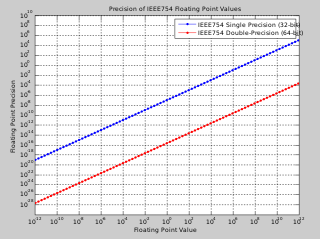
\includegraphics{320px-IEEE754}
  \caption{Precision for different float values}
  \label{prec_value}
\end{figure}

\subsubsection{Wasteful representation}\label{sec:wast-repr}

More than one representation for zero and way too many for NaN

\subsection{POSIT}\label{sec:posit}


\section{Related work}\label{sec:relatedwork}

\subsection{Rational number mathematics}\label{sec:rationalnumbers}

One can calculate most of the fractions using rational representation

\section{Increasing Float size}\label{sec:increasefloat}

Over the years, the number of bits in floating point operations has
increased in order to imrpve number accuracy.


\end{document}
